\section{Lösungskonzept}
Das Lösungskonzept soll von aussen nach innen definiert werden. Darum werden zuerst die Systemgrenzen definiert. Anschliessend werden die Funktionen beschrieben. Diese werden nachfolgend in Teilsysteme unterteilt. Am Schluss wird noch ein alternativer Ansatz diskutiert, der aber nicht weiterverfolgt wird.

\subsection{Systemgrenzen}
Wie dem nachfolgendem Diagramm entnommen werden kann, wird sich das Projekt auf den Dojo konzentrieren. Alle Systeme die es für das Gesamtsystem Museum braucht, sollen nicht betrachtet werden. Es sollen die Schnittstellen soweit definiert werden, dass die Einbindung in ein Gesamtsystem keine Probleme bereiten sollte.

\begin{figure}[H]
\begin{center}
	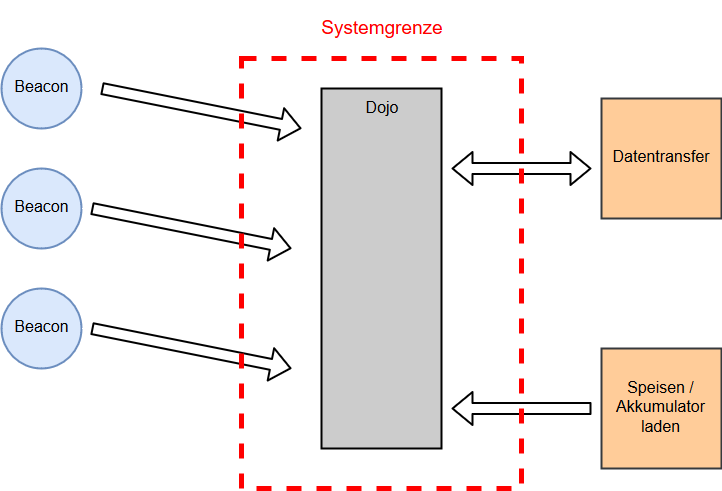
\includegraphics[width=140mm]{data/Loesungskonzept_Systemgrenzen.png}
	\caption{Systemgrenzen des Dojo} %picture caption
	\label{fig:first_layer}
\end{center}
\end{figure}

\subsection{Funktionen}
Die Funktionen sind in zwei Bereiche geteilt. Zum einen sind die Funktionen für die Museumsbesucher beschrieben, welche nachfolgend als Nutzer bezeichnet werden. Zum anderen die für die Museumsbetreiber relevanten Funktionen, diese werden nachfolgend als Betreiber bezeichnet.
\subsubsection*{Nutzer}
Der Nutzer geht mit dem Dojo durch das Museum. Sobald die Bluetooth Beacons genug nahe sind, wird dem Nutzer Signal gesendet. Dies erfolgt durch Vibration oder mithilfe einer LED. Jetzt soll der Nutzer entscheiden ob er das dazugehörige Audio-File sich anhören will. Will er das kann er den Play-Button betätigen. Die Lautstärke kann auch justiert werden mithilfe der Buttons. Falls das Austellungsstück dem Nutzer gefallen hat, kann er die Merken-Taste betätigen. Diese speichert sich das Austellungsstück auf eine Liste auf dem Dojo. Am Ende des Museumsbesuches kann diese Liste ausgewertet werden. Dies fällt aber nicht mehr in unsere Systemgrenzen, wir stellen nur sicher das diese Liste exportiert werden kann.
\subsubsection*{Betreiber}
Der Betreiber muss den Dojo konfigurieren. Dies erfolgt über eine SD-Karte. Diese kann mit dem Computer beladen werden. Nachfolgend wird diese in den Dojo eingeführt. Das Nachladen des Akkumulator erfolgt über eine induktive Ladung. Die nächsten zwei Funktionen sind Wunschziele, die vor allem mit Rücksicht auf die Laufzeit realisiert werden. Den Bluetooth-Reciver könnte man kurzzeitig auf einen Bluetooth Beacon umschalten. Der Betreiber müsste nur noch einen Reciver pro Raum installieren. Damit könnte man die gewünschte HeatMap realisieren. Das zweite wäre die Möglichkeit per Bluetooth einzelne Audiofiles auf den Dojo zu übertragen, um im Falle einer Änderung der Austellung die Liste anzupassen.

\subsection{Teilsysteme}
Das Herzstück des Dojo ist ein NRF52 von Nordic Semiconductor. Dieser besitzt einen integrierten Bluetooth-Stack. Dieser ist Bluetooth Low Energy fähig was benötigt wird um die Beacons zu erkennen. Die Daten werden auf einer SD-Karte gespeichert. Der NRF52 wird die Audiodaten an den Verstärker weitergeben, welcher sie am Körperschallaktor ausgibt. Gespeist wird der Dojo von einem Akku welcher Induktiv geladen wird. Diese Teilsysteme werden in den Nachfolgenden Kapitel noch genauer erläutert.

\begin{figure}[H]
\begin{center}
	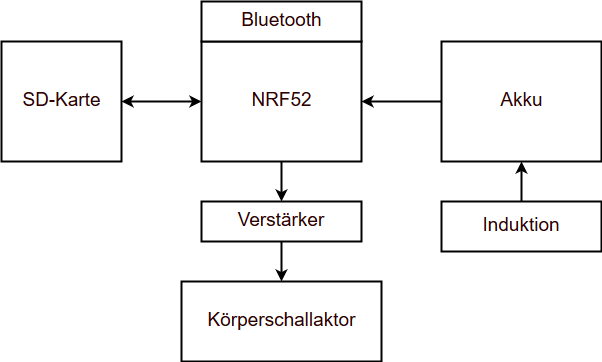
\includegraphics[width=120mm]{data/Loesungskonzept_Teilsysteme.png}
	\caption{Teilsysteme des Dojo} %picture caption
	\label{fig:first_layer}
\end{center}
\end{figure}


\subsection{Alternativer Ansatz}
Im unterstehenden Bild ist unser alternativer Ansatz gezeigt. Es gibt mehrere Gründe die gegen diesen Ansatz sprechen.
\begin{itemize}
\item Der Mux ist schwierig zu realisieren
\item Die SD-Karte über USB zu beladen ist anspruchsvoll
\item Auf den meisten Bluetooth-Modulen(HM-10) ist ein ähnlicher Chip verbaut wie der NRF52
\item Induktives Laden ist spannender als mit USB
\end{itemize}
Diese Gründe und das Gespräch mit Herr Gysin haben uns dazu veranlasst diese Variante zu verwerfen.

\begin{figure}[H]
\begin{center}
	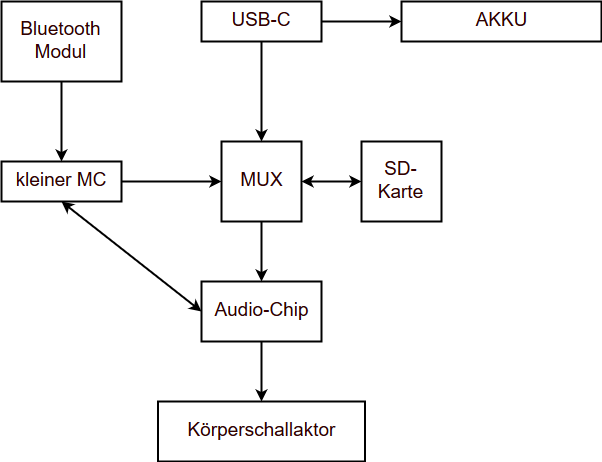
\includegraphics[width=120mm]{data/Loesungskonzept_alternativ.png}
	\caption{Alternatives Lösungskonzept} %picture caption
	\label{fig:first_layer}
\end{center}
\end{figure}


